\chapter{Spatial and temporal relationships between data sources} \label{ch:spatial_and_temporal_relationships}

The second phase of CRISP-DM process model for data mining projects is data understanding;
this chapter discusses the nature of spatial and temporal relationships of different data sources that are used in this master's thesis.
As was discussed in section~\ref{sec:teranet_challenges_solution}, one of the main challenges of working with Teranet's data is the lack of available features.
At the same time, Teranet records have timestamps (dates) and location information (x and y coordinates) and thus can be joined to a variety of other urban data sources, such as Census demographics, Transportation Tomorrow Survey (TTS) and parcel-level land use information.
However, as will be discussed in this chapter, these data sources use different spatial units and are available at different temporal spans;
therefore, special consideration must be taken when joining data from these sources with respect to their temporal and spatial relationships to ensure semantic interoperability.

Different data sources joined to Teranet's dataset are described in this chapter, the implementation of the spatial and temporal relationships via the standardized data preparation workflow in Python and a PostgreSQL relational database are described in chapter~\ref{ch:data_preparation}.

\section{Description of data sources used} \label{sec:description_of_data_sources}

The following data sources were combined into the GTHA housing market database that was created as a part of this master's thesis:

\begin{enumerate}
    \item Teranet's dataset

    Due to the introduction of POLARIS by the Province of Ontario in 1985 (discussed in section~\ref{sec:polaris}), Teranet's dataset includes a complete population of real estate transactions recorded in Ontario from 1985 up to October of 2017 (records prior to 1985 appear to be incomplete, see figure~\ref{fig:teranet_time_series}).
    Since Teranet's dataset has a high number of records, it can be used to investigate aspects relating to the housing market at a very fine spatial and temporal scale.


    \begin{figure}[hbt!]
        \centering
        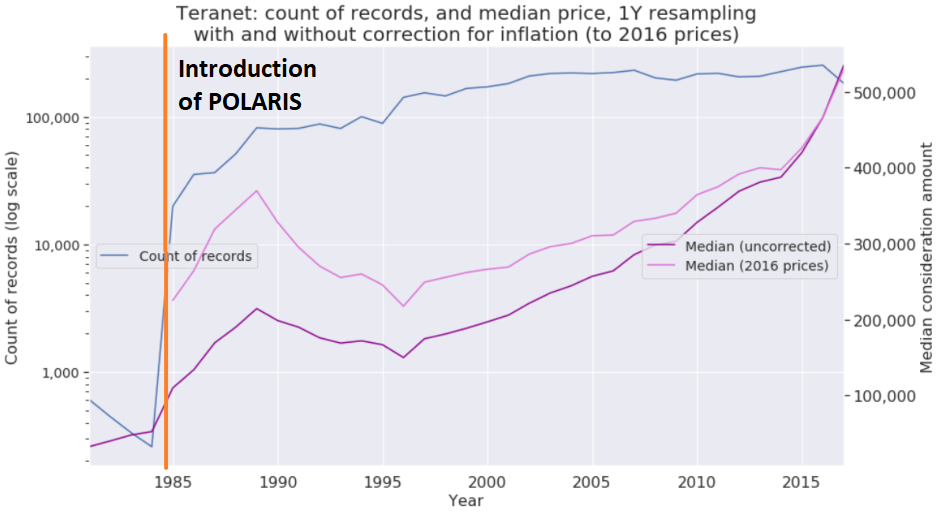
\includegraphics[width=1\linewidth,trim=0 0 0 0,clip]{teranet_time_series.png}
        \caption{Time series of total count of Teranet records within GTHA boundary (log scale, left y-axis) and their median consideration amount (right y-axis), resampled by 1-year intervals.
        It can be seen that there is a dramatic increase in the total count of records between 1984 and 1985, which coincides with the introduction of POLARIS electronic land registration system by the Government of Ontarion in 1985, which was discussed in section~\ref{sec:polaris}.
        Teranet records prior to 1985 appear to be incomplete.}
        \label{fig:teranet_time_series}
    \end{figure}

    \item Select variables from the Census of Canada

    One of the major sources of demographic and statistical data in Canada are the datasets collected under the national Census program.
    Census datasets provide valuable insights into the latest economic, social and demographic conditions and trends in Canada and are used to plan important public services.
    Statistics Canada collects every five years the national Census of Canada and disseminates the information by a range of geographic units, also referred to as "Census geography"\cite{MapandDataLibrary2019}.

    \item Select variables from the Transportation Tomorrow Survey (TTS)

    Another major source of information for most transportation planning studies concerned with Southern Ontario is the Transportation Tomorrow Survey (TTS), an origin-destination travel survey\cite{DataManagementGroup2014}.
    The Transportation Tomorrow Survey (TTS), undertaken every five years since 1986, is a cooperative effort by local and provincial government agencies to collect information about urban travel in southern Ontario.
    TTS represents a retrospective survey of travel taken by every member (age 11 or over) of the household during the day previous to the telephone or web contact.
    The information collected and the method of collection has remained relatively consistent over the seven surveys;
    TTS survey data includes characteristics of the household, characteristics of each person in the household, and details of the trips taken by each member of the household, including details on any trips taken by transit\cite{Ashby2018}.

    \item Land use from DMTI Spatial Inc.\ by year (2001-2014)

    DMTI Spatial Inc., a Digital Map Products company, is a major provider of location based information in Canada.
    DMTI has been providing industry leading enterprise Location Intelligence solutions for more than a decade to Global 2000 companies and government agencies\cite{DMTISpatialInc.2014}.

    \item Detailed land use information from University of Toronto's Department of Geography collected in 2012 and 2013

    The detailed land-use data provided by University of Toronto's Department of Geography is a combination of parcel boundaries (from Teranet) and manually coded land-use data produced using Google maps and streetviews;
    it was collected by Prof.\ Andre Sorensen and Prof.\ Paul Hess's research project.

\end{enumerate}

\section{Spatial relationships between data sources} \label{sec:spatial_relationships}

Most urban areas are divided into zones or planning areas on the basis of maintaining similar population sizes and following built or natural boundaries like roads or rivers.
Census geography follows a certain hierarchy defined by Statistics Canada, with the largest top-level divisions being provinces and territories, and the lowest-tier divisions to which Census data is disseminated being Dissemination Areas (DAs)\cite{StatisticsCanada2018}.
Statistics Canada defines a Dissemination Area as a small area composed of one or more neighbouring dissemination blocks, roughly uniform in population size targeted from 400 to 700 persons to avoid data suppression\cite{StatisticsCanada2015}.

To simulate the changes in accessibility, metropolitan regions are usually broken down into a set of small geographic zones, similar (or in many cases identical) to the set of zones used for regional travel forecasting.
For TTS variables, the finest level of spatial aggregation is that of the Traffic Zone, also referred to as the Traffic Analysis Zone (TAZ).
A Traffic Zone is a polygon which typically falls along the centre line of roads or the natural geographic boundaries\cite{DataManagementGroup2019}.
Not as a rule, but TAZ zones roughly follow Census tract boundaries, which are slightly bigger than DA boundaries.
Figure~\ref{fig:da_taz_difference} presents an example of TAZ polygons overlaid with Census DA boundaries.

\begin{figure}[hbt!]
    \centering
    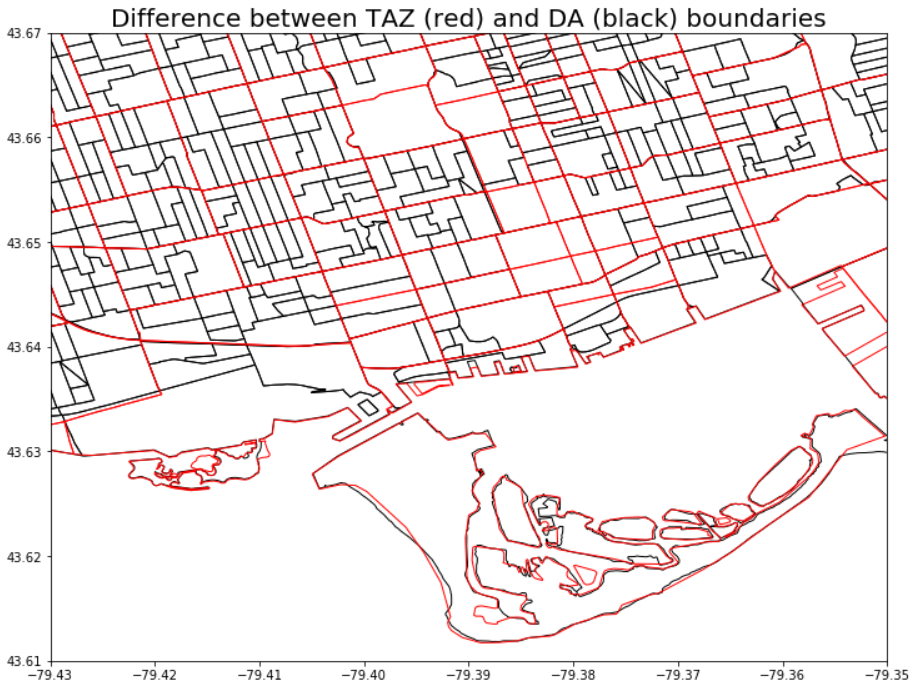
\includegraphics[width=0.7\linewidth,trim=0 0 0 0,clip]{da_taz_difference.png}
    \caption{Spatial relationship between datasets: difference between Traffic Analysis Zones (TAZ, red) and Census Dissemination Area (DA, black).}
    \label{fig:da_taz_difference}
\end{figure}

TTS data has been collected for changing TAZ boundaries, or in other words, different zone systems due to growing population and expanding extents of the survey in the GTHA region over the years.
To make the TTS data consistent for comparing over all years from 1986 to 2016, the Data Management Group (DMG) at the University of Toronto Transportation Research Institute (UTTRI), the custodian of the dataset derived from TTS, made all surveys available in the 2001 zone system, for convenience of researchers (any zone system could have been chosen for that matter).
UTTRI used the 2001 TAZ system to model travel times for the GTHA on EMME for all TTS years based on the origin-destination trip data collected in the survey.
The travel time data was used to create further transportation accessibility variables.

Land use data collected by DMTI and by the Department of Geography uses the spatial unit of a parcel polygon.
Teranet records have attributes representing x and y coordinates matching parcel centroids.

\vspace{5mm}

Below is the summary of spatial units used by the data sources that were combined into the GTHA housing market database, designed and implemented as a part of this master's thesis:

\begin{itemize}
    \item Point data
    \begin{itemize}
        \item Teranet
    \end{itemize}
    \item Parcel-level data (polygons)
    \begin{itemize}
        \item detailed land use from the Department of Geography
        \item land use from DMTI
    \end{itemize}
    \item DA-level data (polygons)
    \begin{itemize}
        \item Census variables
    \end{itemize}
    \item TAZ-level data
    \begin{itemize}
        \item TTS variables
    \end{itemize}
\end{itemize}

When joining these data sources, difference in spatial units needs to be respected, which can be more challenging when spatially joining polygons with polygons, since it might require area-weighted spatial interpolation of data to a common unit of analysis.
In addition, polygon-based data can also vary with time, as is the case with DMTI's land use information, which is available by year.
To simplify relating different polygon-based data sources with each other, all of them can be brought together to a single level of time-indexed points, such as Teranet transactions.
This allows flexibility in combining data from polygon-based data sources to a common point level while maintaining the integrity of spatial and temporal relationships through polygon-to-point spatial joins.
Implementation of these relationships is described in chapter~\ref{ch:data_preparation}, temporal relationships between different data sources are described in the following section.

\section{Temporal relationships between data sources} \label{sec:termporal_relationships_between_datasets}

In addition to using different spatial units, data sources joined with Teranet's dataset are available at different temporal spans:
\begin{itemize}
    \item Teranet records have individual timestamps (date) on each record
    \item Census and TTS variables are sampled once in 5 years
    \item DMTI's land use data is available by year and covers a time span from 2001 to 2014
    \item Detailed land use from the Department of Geography was collected at a single point in time during the summers of 2012 and 2013
\end{itemize}

Temporal matching between Teranet records and DMTI data can be done directly: DMTI land use for each year from 2001 to 2014 can be spatially joined with a subset of Teranet records from the corresponding year;
such approach would ignore changes of land use types that occur within a year, but would recognize land use changes between the years for which DMTI land use data is available.
Since the detailed land use provided by the Department of Geography was collected at a single point in time, it can be joined to all Teranet records;
however, it should be kept in mind that this land use data will be the most accurate around its time of collection in 2012 and 2013, and will become increasingly less accurate with an increase of the temporal span of Teranet records.

\begin{figure}[hbt!]
    \centering
    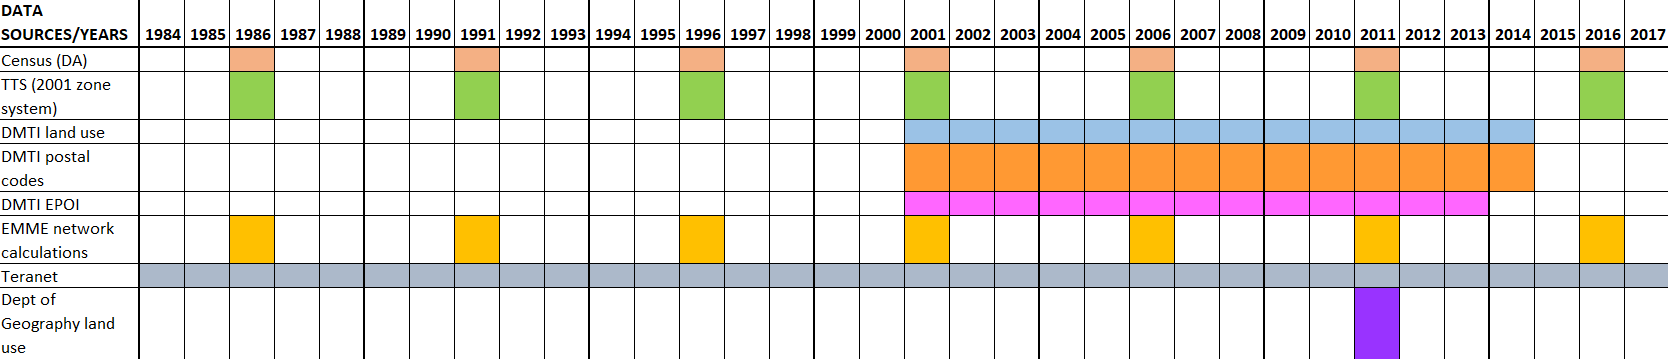
\includegraphics[width=1\linewidth,trim=0 0 0 0,clip]{temporal_spans.png}
    \caption{Temporal spans of data sources used in the GTHA housing market database.}
    \label{fig:temporal_spans}
\end{figure}

\vspace{5mm}

As for Teranet and Census / TTS variables, they can be matched in a number of ways:

\begin{enumerate}
    \item Direct match with appropriate Teranet subsets
    \begin{itemize}
        \item match Census / TTS variables only with Teranet records from the corresponding year (for example, Teranet records from 2016 matched with 2016 Census / TTS variables)
        \item benefits:
        \begin{itemize}
            \item Census / TTS variables would be composed of the actual values recorded by the survey
        \end{itemize}
        \item disadvantages:
        \begin{itemize}
            \item limited use of Teranet data since only records from Census / TTS years can be matched
        \end{itemize}
    \end{itemize}
    \item Interpolation of discrete Census / TTS variables
    \begin{itemize}
        \item discrete Census / TTS variables can be turned into continuous via interpolation
        \item benefits:
        \begin{itemize}
            \item closest temporal match between Teranet and Census / TTS variables
        \end{itemize}
        \item disadvantages:
        \begin{itemize}
            \item additional assumptions need to be made for each Census / TTS variable
        \end{itemize}
    \end{itemize}
    \item Assign temporal spans to each Census / TTS survey as new features to Teranet records
    \begin{itemize}
        \item each Census / TTS survey is assigned a temporal span of 5 years;
        this 5-year span represents a group of Teranet records to which variables from this survey can be matched (for example, Census variables of 2016 are matched with Teranet record from 2014 to 2018)
        \item benefits:
        \begin{itemize}
            \item avoid interpolation assumptions
        \end{itemize}
        \item disadvantages:
        \begin{itemize}
            \item step-change in Census / TTS variables
        \end{itemize}
    \end{itemize}
\end{enumerate}

To avoid additional interpolation assumptions and use the actual values recorded from Census and TTS surveys, the third option has been chosen for matching Teranet records with Census / TTS variables.
Each Census / TTS survey is assigned a 5-year time span centered at the survey year (i.e., 2014--2018 for 2016 survey year) and new foreign keys are introduced to Teranet records to allow matching with 5-year time spans of Census / TTS variables.
Implementation of temporal relationships for Teranet records will be described in chapter~\ref{ch:data_preparation}.
Figure~\ref{fig:temporal_spans} presents the temporal spans assigned to each data source for joining with Teranet records.

\section{Chapter summary} \label{sec:data_sources_summary}

Variables that can be joined to augment Teranet's dataset, such as Census and TTS surveys and parcel-level land use data, are defined using different spatial units and are available at varying temporal spans.
These relationships need to be respected when combining variables from these data sources into a single dataset to ensure semantic interoperability.
The integrity of spatial relationships can be ensured by spatially joining all polygon-based data sources to Teranet points.
Temporal relationships between DMTI land use and Teranet sales records are incorporated by performing separate spatial join operations for each annual DMTI land use dataset with a corresponding Teranet subset.
For Census and TTS variables, additional foreign keys are introduced assigning 5-year spans to each Teranet record corresponding to a Census / TTS survey;
these foreign keys indicate which Teranet records should be joined to a particular Census or TTS survey.
Implementation of these relationships via a standardized data preparation workflow in Python and a PostgreSQL relational database are described in chapter~\ref{ch:data_preparation}.
